\documentclass[a4paper,11pt]{article}
\usepackage{exptech}
\usepackage{textcomp}
\usepackage{graphicx}
\usepackage{array}
\usepackage[babel=true]{csquotes}
\usepackage{url}
\usepackage{hyperref}
\usepackage{wrapfig}
\usepackage[export]{adjustbox}
\usepackage{titletoc}

\hypersetup{
  bookmarks=true, % show bookmarks bar?
  pdftitle={Avalon - Rapport de pré-étude}, % title
  pdfnewwindow=true, % links in new window
  colorlinks=true, % false: boxed links; true: colored links
  linkcolor=black, % color of internal links (change box color with linkbordercolor)
  citecolor=cyan, % color of links to bibliography
  filecolor=cyan, % color of file links
  urlcolor=cyan % color of external links
}

\title{
  \textbf{Avalon}\\
  Rapport de pré-étude
}
\markright{Avalon - Rapport de pré-étude}
\author{
\begin{minipage}{0.4\textwidth}
	\begin{flushleft} \large
		\emph{Auteurs :}\\
		Alexandre \textsc{Audinot}\\
		Julien \textsc{Bouvet}\\
		Cyrille \textsc{Delabre}\\
		Thierry \textsc{Gaugry}\\
		Nicolas \textsc{Hurman}\\
		Léo \textsc{Jacoboni}\\
		Alexandre \textsc{Leonardi}\\
	\end{flushleft}
\end{minipage}
\begin{minipage}{0.4\textwidth}
	\begin{flushright} \large
		\emph{Encadrants :} \\
		Valérie \textsc{Gouranton}\\
		Ronan \textsc{Gaugne}\\
		Bruno \textsc{Arnaldi}\\
		Willy \textsc{Allègre}\\
		Jean-Paul  \textsc{Departe}\\
	\end{flushright}
\end{minipage}
}

\date{23 octobre 2014}

\begin{document}
\maketitle
\thispagestyle{empty}
\begin{abstract}
\textbf{Avalon :} Environnement de Réalité Virtuelle pour l'apprentissage à l'utilisation d'appartements tremplins. Réalisation en 3D d'un appartement domotisé interactif utilisé dans le cadre de la rééducation des personnes handicapées.
Le projet est proposé par le centre mutualiste de rééducation et de réadaptation fonctionnelles de Kerpape (plus particulièrement les ingénieurs du laboratoire électronique Willy Allègre et Jean-Paul Departe).
Le modèle 3D de l'appartement nous est fourni, et notre travail consistera à réaliser un logiciel fonctionnel permettant de se déplacer dans l'appartement et implémentant les interactions avec les différents éléments de domotiques, en plus de prendre en charge différents périphériques de contrôle. 
\end{abstract}

\begin{figure}[h!]
	\centering
	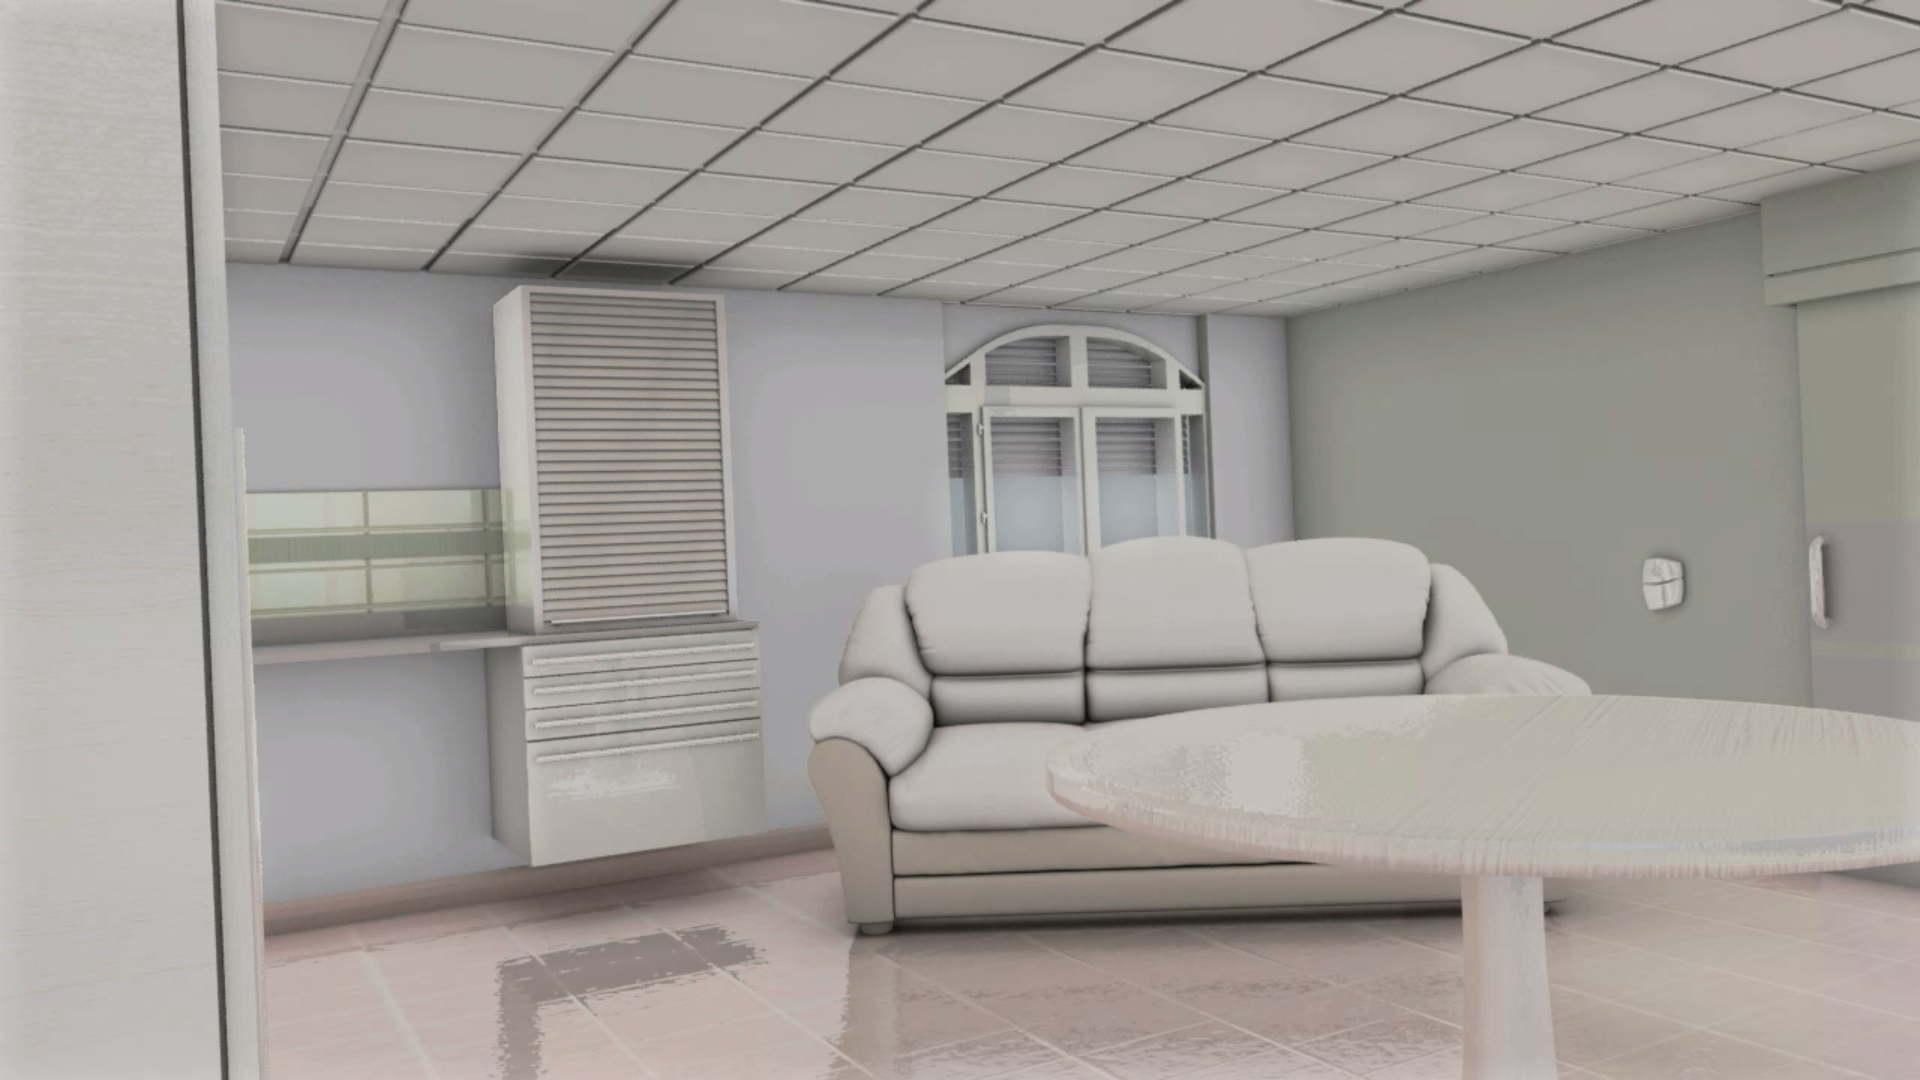
\includegraphics[height=170pt]{6-Documentation/img/screen_appart.png}
\end{figure}

%\vfill
%[width=\textwidth]
\begin{figure}[h!]
   \begin{minipage}{0.3\linewidth}
      
\includegraphics[scale=0.9]{6-Documentation/img/logo_insa.jpeg}
   \end{minipage} 
   \begin{minipage}{0.2\linewidth}
      \centering
      
\includegraphics[scale=0.5,left]{6-Documentation/img/logo_irisa.jpg}
   \end{minipage}\hfill
   \begin{minipage}{0.2\linewidth}
      
\includegraphics[scale=0.9]{6-Documentation/img/logo_kerpape.png}
   \end{minipage}
\end{figure}

\pagebreak

\tableofcontents
\pagebreak


\end{document}
